% ---------------------------------------------------------------------------
% Relazione di progetto
% Automazione dei sistemi elettrici di trasporto - Politecnico di Milano
%
% Come si usa:
%   1. Il testo in latino e' un segnaposto: si sostituisce, sezione per sezione.
%      La struttura (le sezioni) NON si cambia.
%   2. Le figure stanno in figure/: sostituite figura-1.png e figura-2.png con
%      le vostre, stesso nome oppure cambiate il nome in \includegraphics.
%   3. Le fonti vanno in bibliografia.bib e si citano con \cite{chiave}.
%   4. Compilare: su Overleaf caricate l'intera cartella relazione/ (zip) e
%      premete Recompile; in locale, "latexmk -pdf relazione.tex" oppure
%      "tectonic relazione.tex".
%   5. Si consegna il PDF.
% ---------------------------------------------------------------------------
\documentclass[conference]{IEEEtran}

\usepackage[utf8]{inputenc}
\usepackage[T1]{fontenc}
\usepackage[italian]{babel}
\usepackage{graphicx}
\usepackage{amsmath}
\usepackage{booktabs}
\usepackage{siunitx}
\DeclareSIUnit{\euro}{\text{\texteuro}}
\usepackage{url}
\usepackage[hidelinks]{hyperref}

\graphicspath{{figure/}}

\begin{document}

\title{Titolo del progetto: una riga che dice cosa avete fatto}

% Un blocco \IEEEauthorblockN / \IEEEauthorblockA per ogni componente del gruppo.
\author{
  \IEEEauthorblockN{Nome Cognome}
  \IEEEauthorblockA{Matricola 000000\\
  Politecnico di Milano\\
  nome.cognome@mail.polimi.it}
  \and
  \IEEEauthorblockN{Nome Cognome}
  \IEEEauthorblockA{Matricola 000000\\
  Politecnico di Milano\\
  nome.cognome@mail.polimi.it}
  \and
  \IEEEauthorblockN{Nome Cognome}
  \IEEEauthorblockA{Matricola 000000\\
  Politecnico di Milano\\
  nome.cognome@mail.polimi.it}
}

\maketitle

\begin{abstract}
% 150-200 parole, da scrivere per ultime: problema, cosa avete fatto, cosa avete
% trovato. Niente promesse: solo quello che c'e' davvero nella relazione.
Lorem ipsum dolor sit amet, consectetur adipiscing elit. Sed do eiusmod tempor
incididunt ut labore et dolore magna aliqua. Ut enim ad minim veniam, quis
nostrud exercitation ullamco laboris nisi ut aliquip ex ea commodo consequat.
Duis aute irure dolor in reprehenderit in voluptate velit esse cillum dolore eu
fugiat nulla pariatur. Excepteur sint occaecat cupidatat non proident, sunt in
culpa qui officia deserunt mollit anim id est laborum.
\end{abstract}

\begin{IEEEkeywords}
% 4-6 termini, separati da virgola.
mobilit\`a elettrica, ricarica, automazione, parola chiave, parola chiave
\end{IEEEkeywords}

\section{Introduzione}
% Qual e' il problema, perche' conta, cosa avete fatto voi. Ultimo capoverso:
% come e' organizzata la relazione.
Lorem ipsum dolor sit amet, consectetur adipiscing elit. Sed do eiusmod tempor
incididunt ut labore et dolore magna aliqua. Ut enim ad minim veniam, quis
nostrud exercitation ullamco laboris nisi ut aliquip ex ea commodo consequat.

Duis aute irure dolor in reprehenderit in voluptate velit esse cillum dolore eu
fugiat nulla pariatur. Excepteur sint occaecat cupidatat non proident, sunt in
culpa qui officia deserunt mollit anim id est laborum.

La relazione \`e organizzata cos\`i: la Sezione~\ref{sec:stato} riassume lo
stato dell'arte, la Sezione~\ref{sec:metodo} descrive il metodo, la
Sezione~\ref{sec:risultati} presenta i risultati, la Sezione~\ref{sec:limiti}
li discute.

\section{Stato dell'arte}
\label{sec:stato}
% Cosa esiste gia': normativa, letteratura, prodotti sul mercato. Ogni
% affermazione non ovvia va appoggiata a una fonte, cosi': \cite{chiave}.
Lorem ipsum dolor sit amet, consectetur adipiscing elit~\cite{esempio2025}.
Sed do eiusmod tempor incididunt ut labore et dolore magna aliqua. Ut enim ad
minim veniam, quis nostrud exercitation ullamco laboris nisi ut aliquip ex ea
commodo consequat. Duis aute irure dolor in reprehenderit in voluptate velit
esse cillum dolore eu fugiat nulla pariatur.

\section{Metodo}
\label{sec:metodo}
% Cosa avete fatto e come, con abbastanza dettaglio perche' un altro gruppo
% possa rifarlo: dati, ipotesi, strumenti, modello.
Lorem ipsum dolor sit amet, consectetur adipiscing elit. Il costo annuo di
percorrenza si calcola come
\begin{equation}
  C = \frac{d}{100}\, c \, p ,
  \label{eq:costo}
\end{equation}
dove $d$ \`e la percorrenza annua in \si{\kilo\metre}, $c$ il consumo per
\SI{100}{\kilo\metre} e $p$ il prezzo unitario dell'energia. La
Figura~\ref{fig:schema} mostra lo schema del sistema.

\begin{figure}[t]
  \centering
  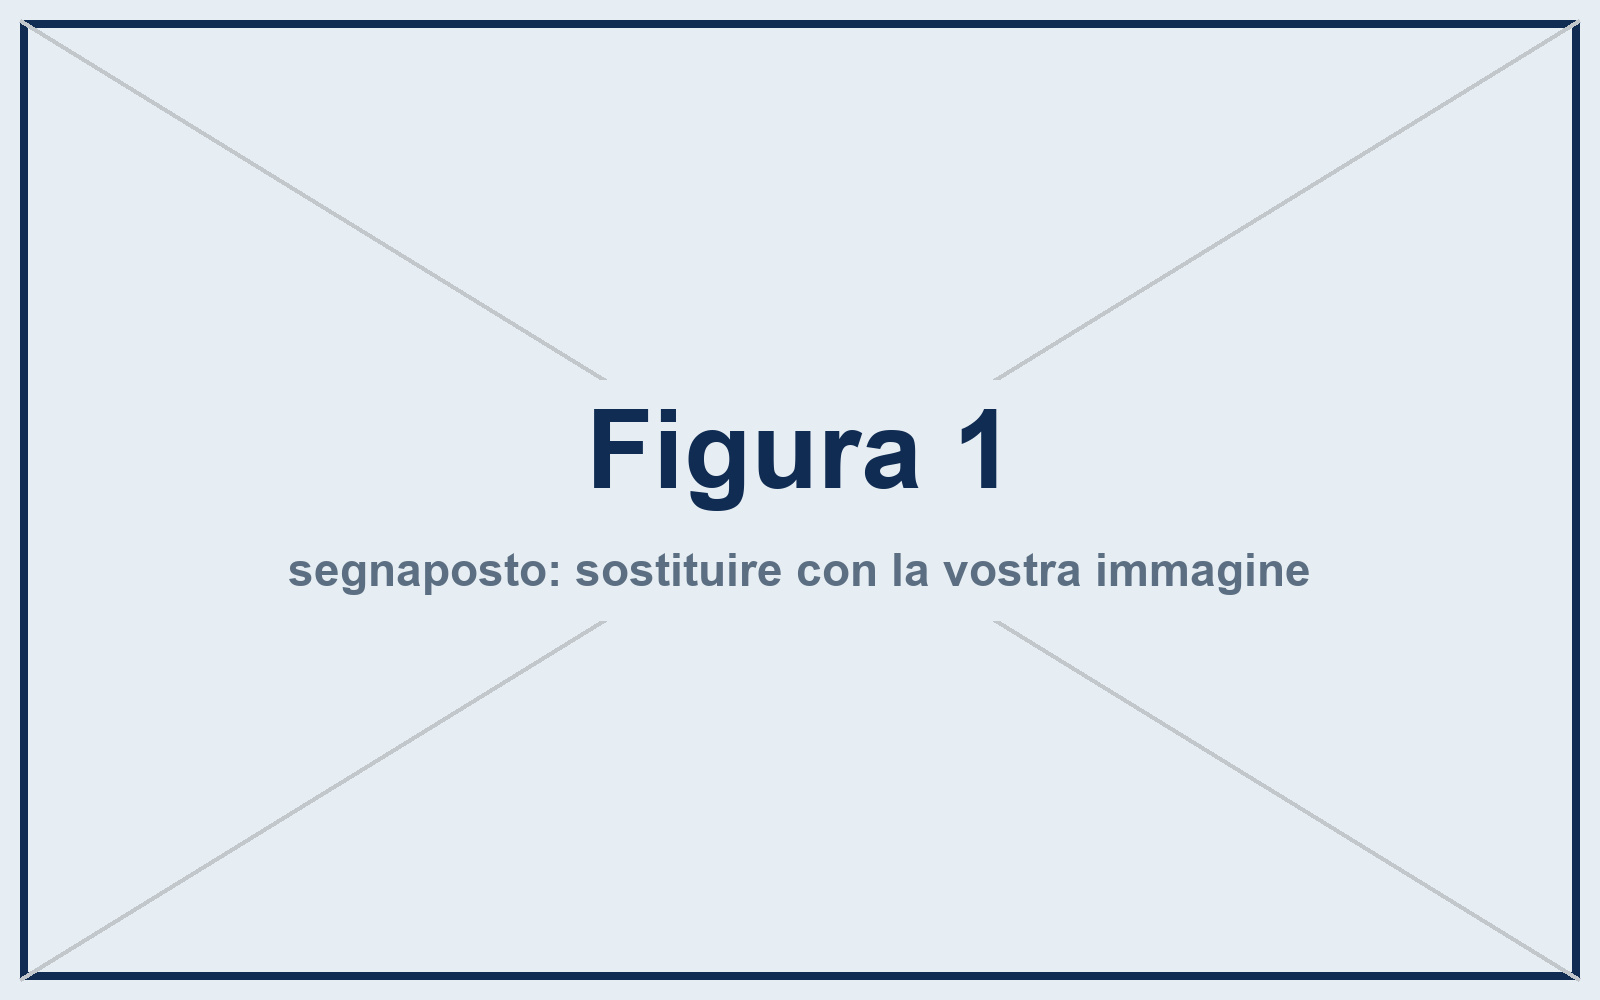
\includegraphics[width=\columnwidth]{figura-1.png}
  \caption{Didascalia della figura: dice cosa si deve guardare, non solo cosa
  c'\`e. Segnaposto da sostituire.}
  \label{fig:schema}
\end{figure}

Ut enim ad minim veniam, quis nostrud exercitation ullamco laboris nisi ut
aliquip ex ea commodo consequat. I parametri usati sono in
Tabella~\ref{tab:parametri}.

\begin{table}[t]
  \caption{Parametri del caso di studio (valori di esempio).}
  \label{tab:parametri}
  \centering
  \begin{tabular}{lS[table-format=5.2]l}
    \toprule
    Parametro & {Valore} & Unit\`a \\
    \midrule
    Percorrenza annua      & 15000 & \si{\kilo\metre} \\
    Consumo auto termica   & 6.5   & \si{\litre}/\SI{100}{\kilo\metre} \\
    Prezzo benzina         & 1.75  & \si{\euro}/\si{\litre} \\
    Consumo auto elettrica & 18    & \si{\kilo\watt\hour}/\SI{100}{\kilo\metre} \\
    Prezzo energia         & 0.25  & \si{\euro}/\si{\kilo\watt\hour} \\
    \bottomrule
  \end{tabular}
\end{table}

\section{Risultati}
\label{sec:risultati}
% I numeri, le figure e le tabelle. Commentateli: una figura senza una frase
% che dica cosa si deve guardare non serve a niente.
Con i parametri di Tabella~\ref{tab:parametri} e l'equazione~\eqref{eq:costo},
il costo annuo risulta di \SI{1706}{\euro} per l'auto termica e di
\SI{675}{\euro} per quella elettrica. La Figura~\ref{fig:risultati} mostra
come varia il risparmio al variare della percorrenza.

\begin{figure}[t]
  \centering
  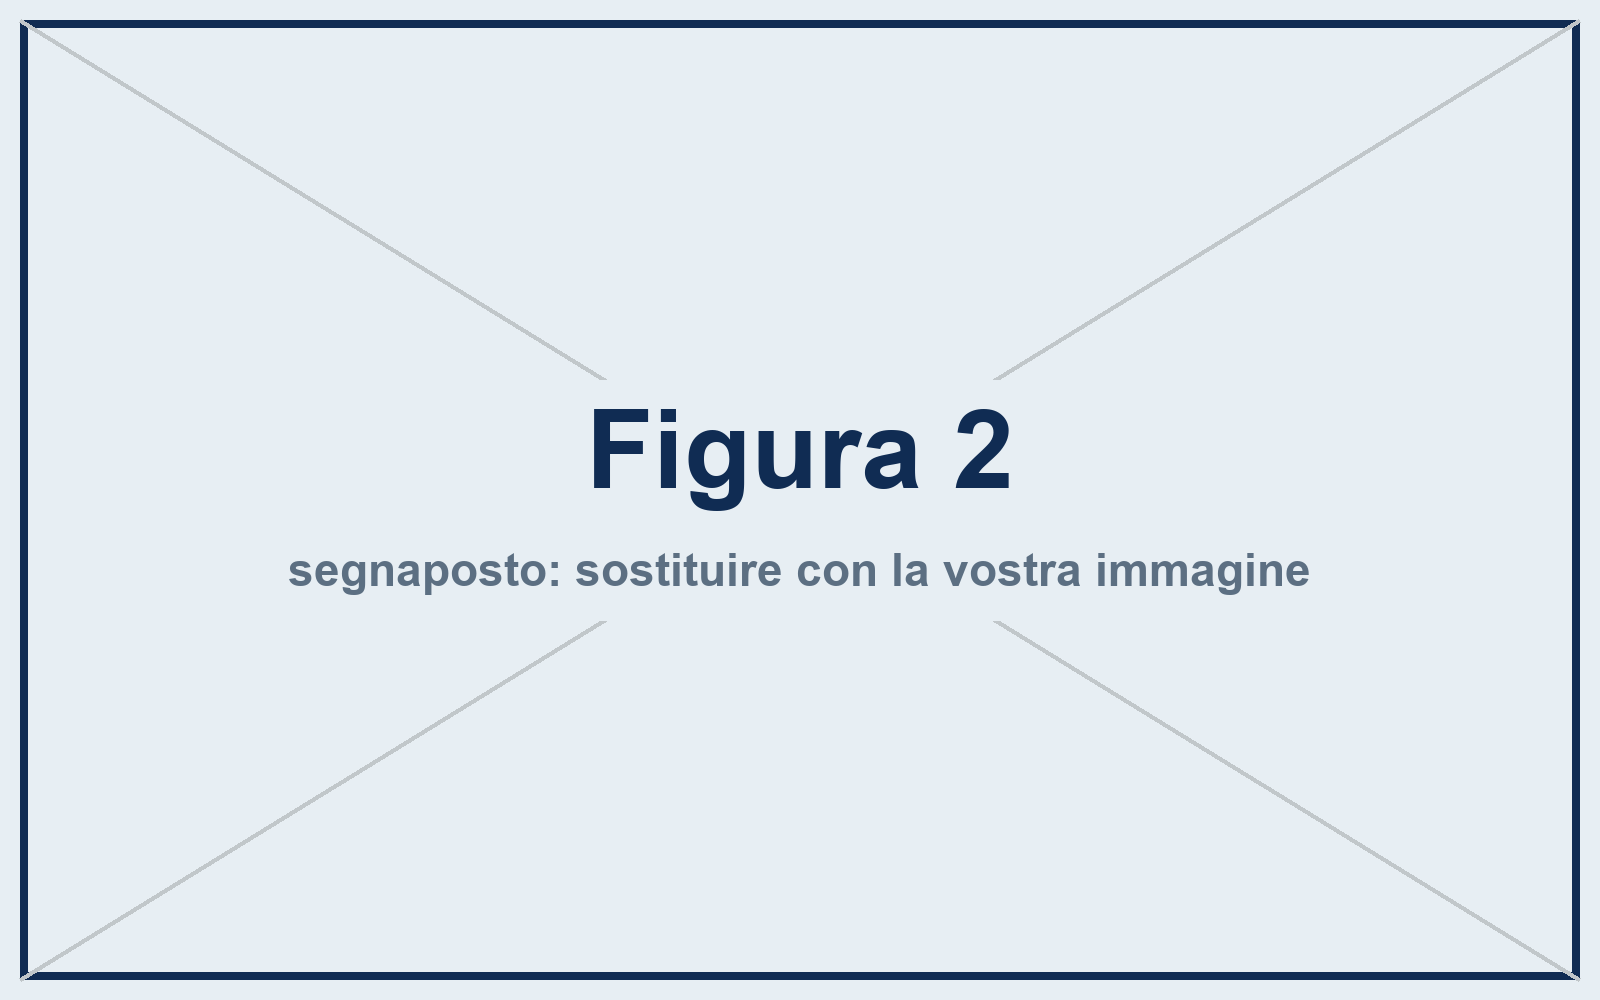
\includegraphics[width=\columnwidth]{figura-2.png}
  \caption{Seconda figura segnaposto: da sostituire con un grafico vero.}
  \label{fig:risultati}
\end{figure}

Lorem ipsum dolor sit amet, consectetur adipiscing elit. Sed do eiusmod tempor
incididunt ut labore et dolore magna aliqua.

\section{Discussione e limiti}
\label{sec:limiti}
% Cosa significano i risultati, dove il metodo non regge, cosa serve per
% andare oltre. I limiti dichiarati valgono piu' di quelli nascosti.
Lorem ipsum dolor sit amet, consectetur adipiscing elit. Sed do eiusmod tempor
incididunt ut labore et dolore magna aliqua. Ut enim ad minim veniam, quis
nostrud exercitation ullamco laboris nisi ut aliquip ex ea commodo consequat.

\section{Conclusioni}
% Tre o quattro frasi. Niente idee nuove qui dentro.
Lorem ipsum dolor sit amet, consectetur adipiscing elit. Sed do eiusmod tempor
incididunt ut labore et dolore magna aliqua.

\section*{Uso di strumenti di intelligenza artificiale}
% Obbligatoria. Quale agente avete usato, per fare cosa, e come avete
% verificato quello che ha prodotto.
Lorem ipsum dolor sit amet, consectetur adipiscing elit. Sed do eiusmod tempor
incididunt ut labore et dolore magna aliqua.

% --- Bibliografia -----------------------------------------------------------
% Le voci stanno in bibliografia.bib. Questa riga le mette in ordine di citazione.
\bibliographystyle{IEEEtran}
\bibliography{bibliografia}

\end{document}
